In this section, the proposed \TAIL{} agent is introduced.
The architecture of the proposed agent is the same as \DAIL{}, which is illustrated in Figure \ref{ch:TAIL:fig:Architecture}.
It is important to note that the loss functions for three deep feed-forward networks $F$, $G$, and $D$ are similar to the \DAIL{} agent.
The only difference is that the \TAIL{} agent is trained on both source and target tasks simultaneously and under the same domain.
Thus, instead of extracting domain-shared and domain-specific features, \TAIL{} is trained to learn the similarities and differences between source and target tasks.

\begin{figure}[H]
  \centering
  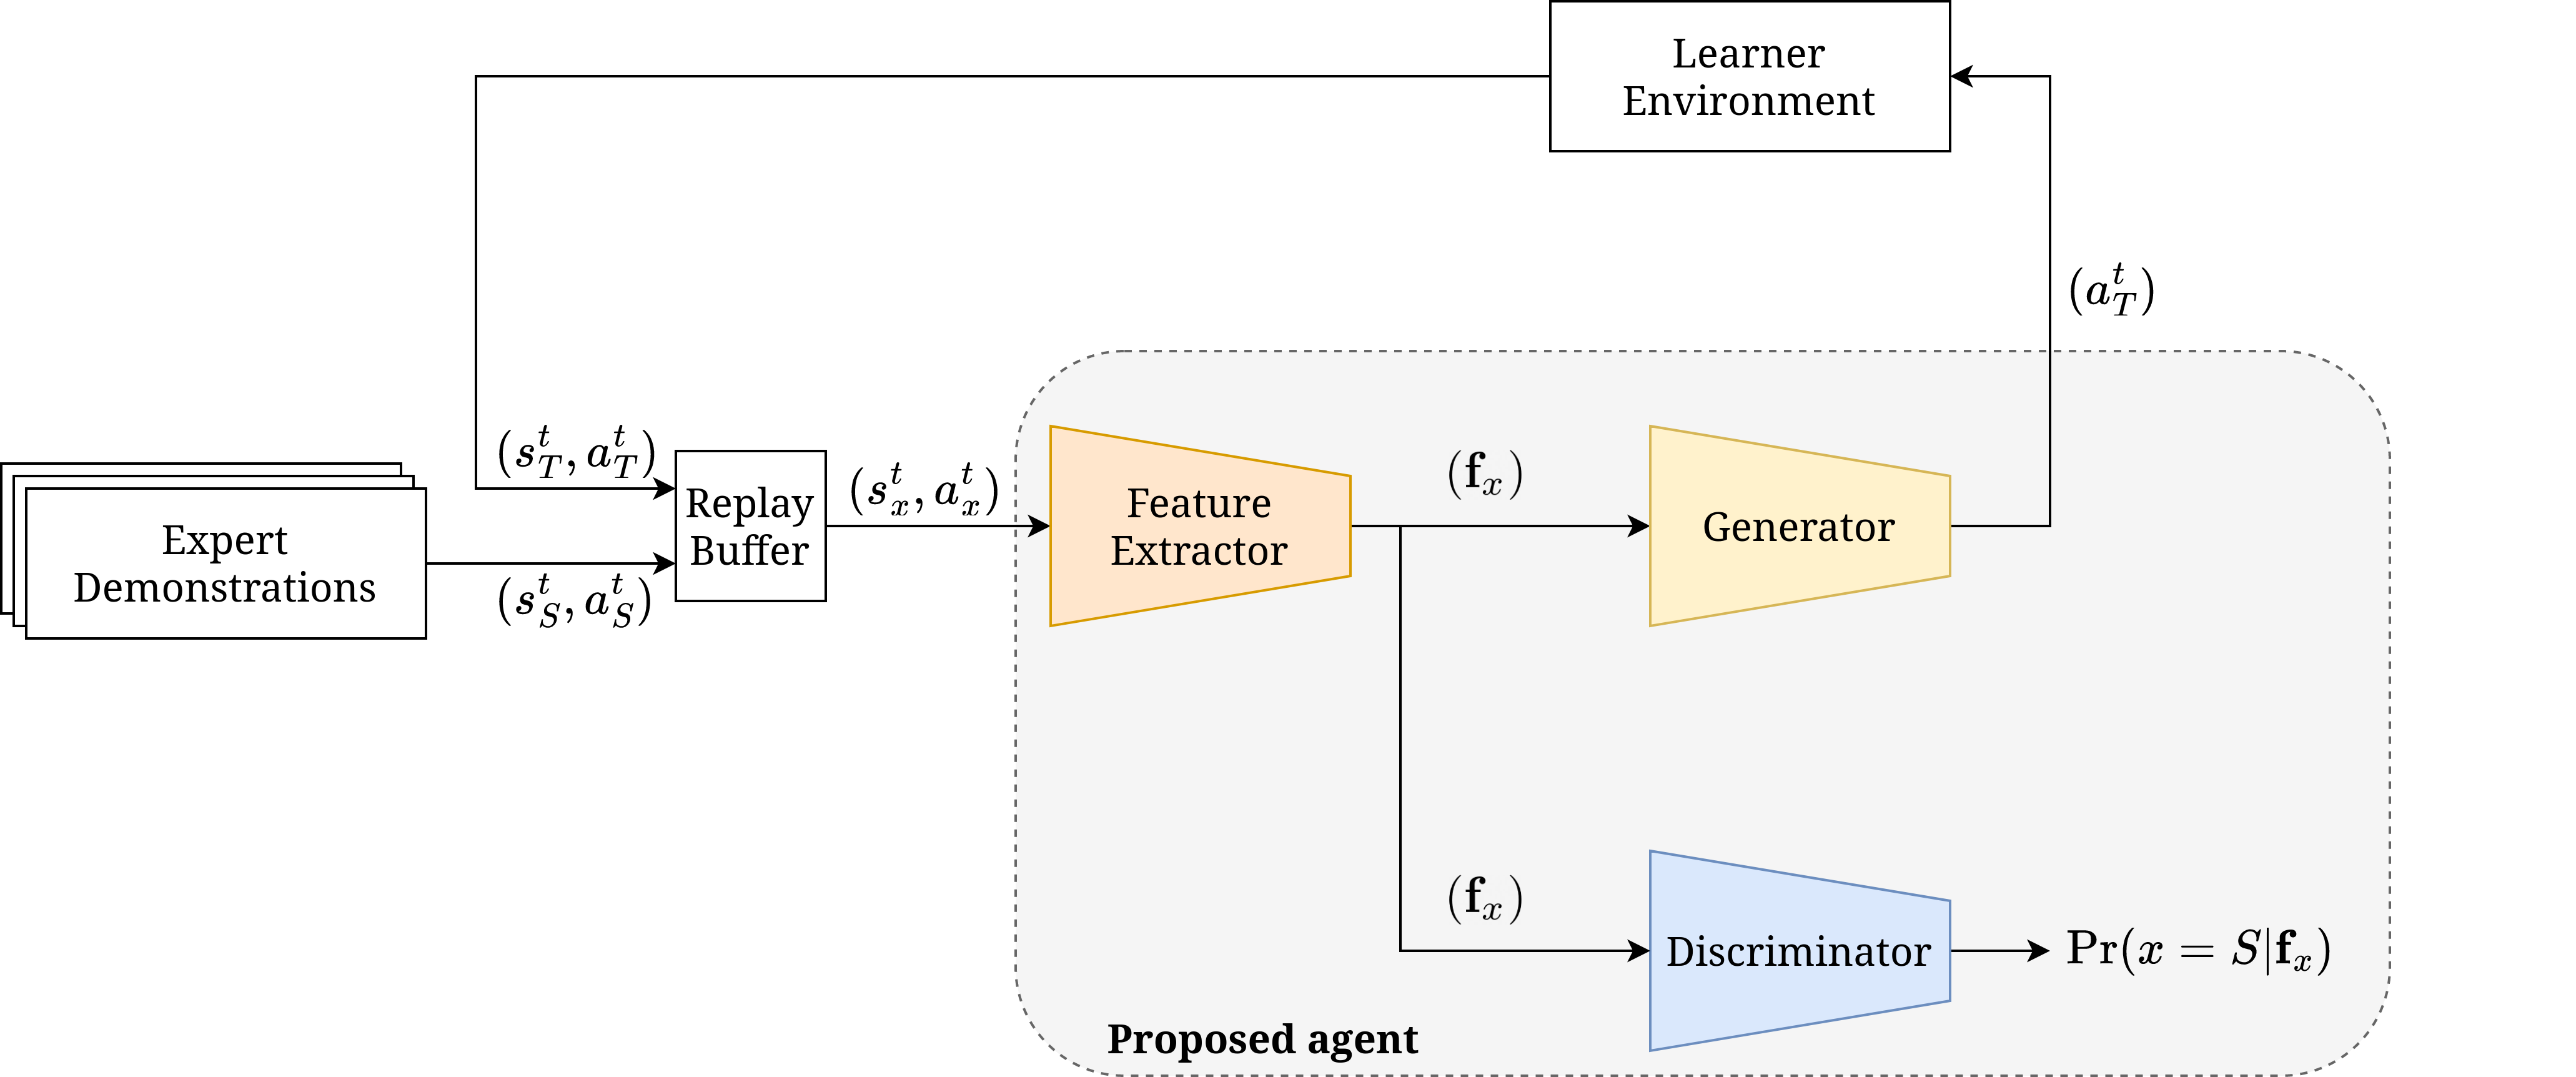
\includegraphics[width=0.9\linewidth]{\FigsDir/new_Architecture.png}
  \caption{\added{The neural network architecture of the proposed \TAIL{} agent.}\label{ch:TAIL:fig:Architecture}}
\end{figure}

\subsection{Feature Extractor Network \texorpdfstring{$F$}{F}}
A state-action pair $(s^t_x, a^t_x)$ in task $x$ is \added{sampled from a replay buffer \cite{zhang2017deeper} and} input to the feature extractor $F$ to produce a feature vector $\mathbf{f}_x=F(s^t_x, a^t_x)$.
$F$ is trained to capture the structural similarities or differences between source $\mathbb{M}^-_S$ and target $\mathbb{M}^-_T$ tasks by minimizing the distance between two features $\mathbf{f}_S$ and $\mathbf{f}_T$.
Therefore, the loss function of $F$ is defined as:

\begin{align}
  \mathfrak{L}_F (F, G) & = \mathbb{E} \left[ \left\|
    F(s^t_S, a^t_S) - F(s^t_T, a^t_T)
  \right\| \right]                                    \\
                        & = \mathbb{E} \left[ \left\|
    F(s^t_S, a^t_S) - F( s^t_T, G( F( s^t_S, a^t_S ) ) )
    \right\| \right]
  % 1/T \sum^{}_{}{|| f() - f() ||^2_2}
\end{align}


\subsection{Discriminator Network \texorpdfstring{$D$}{D} and Generator Network \texorpdfstring{$G$}{G}}

The discriminator $D$ is designed to distinguish between $\mathbf{f}_S$ and $\mathbf{f}_T$.
Specifically,
$D$ receives a feature vector $\mathbf{f}_x$ outputs a probability $\mathrm{Pr}(x=S|\mathbf{f}_x)$ to classify whether $\mathbf{f}_x$ is from source $\mathbb{M}^-_S$ or target $\mathbb{M}^-_T$ tasks.
Meanwhile,
the generator $G$ aims to generate an action $a^t_T$ so that $\mathbf{f}_T = F(s^t_T, a^t_T)$ looks as similar as possible to $\mathbf{f}_S$.
In the proposed \DAIL{} agent,
the adversarial loss \cite{GAN_Original} is applied for both networks:

\begin{align}
  \mathfrak{L}_{GAN}(G, D) & =
  \mathbb{E}[
    \log{D(F(s^t_S, a^t_S))}
  ] + \mathbb{E}[
    \log{(1-D(F(s^t_T, a^t_T)))}
  ]                                        \\
                           & = \mathbb{E}[
    \log{D(F(s^t_S, a^t_S))}
  ] + \mathbb{E}[
    \log{(1-D(F(s^t_T, G(F(
      s^t_S, a^t_S
      )))))}
  ]
\end{align}

The optimal policy is achieved using a RL-based policy gradient,
which relies on reward signal $r=-\log{D(F(s^t_S, a^t_S))}$ provided by the learned discriminator.


\subsection{Full Objective}

During the learning phase,
in order to capture the similarities and differences between source and target tasks,
the feature extractor $F$ and the generator $G$ are optimized to minimize the feature extractor loss $\mathfrak{L}_F$.
At the same time,
given a feature vector $\mathbf{f}_x$ of task $x$,
we want to judge whether $\mathbf{f}_x$ is from $\mathbb{M}^-_S$ or $\mathbb{M}^-_T$ by minimizing the task classification loss $\mathfrak{L}_{GAN}$.
This encourages task-specific features to be captured by $F$.
Overall, the full objective function is:

\begin{align}
   & \underset{F, G}{max} \underset{D}{min} \mathfrak{L}(F, G, D) \\
   & \quad\text{subject to \:}
  \mathfrak{L}(F, G, D) = {\mathfrak{L}_{GAN}(G, D)} - \lambda\mathfrak{L}_F
\end{align}

The learning algorithm of the proposed agent is outlined in Algorithm \ref{ch:TAIL:alg:ProposedModel}.

\begin{algorithm}
  \caption{\TAIL{}}
  \label{ch:TAIL:alg:ProposedModel}

  \begin{algorithmic}[1]
    \Input
    \Desc{$\mathcal{D}_\mathcal{S}$}{A set of expert demonstrations on source tasks}
    \EndInput

    \State Randomly initialize feature extractor network $F$, generator $G$ and discriminator $D$
    \For {i = 0, 1, 2, ...}
    \State Sample an expert demonstration $\tau^i_S \sim \mathcal{D}_S$
    \State Update the parameters of feature extractor network $F$ with the gradient
    \[\mathbf{E}[
        \nabla_F log(D( \mathbf{f}_S ))
      ] + \mathbf{E}[
        \nabla_F log(1 - D( \mathbf{f}_T ))
      ] - \lambda \mathbf{E}[
        \nabla_F \left\|
        \mathbf{f}_S - \mathbf{f}_T
        \right\|
      ]
    \]
    \State Update the discriminator parameters with the gradient
    \[\mathbf{E}[
        \nabla_D log(D( \mathbf{f}_S ))
      ] + \mathbf{E}[
        \nabla_D log(1 - D( \mathbf{f}_T ))
      ]\]
    \State Update policy $\pi_{L}$ with the reward signal $r=-logD(\mathbf{f}_S)$
    \EndFor

    \Output
    \Desc{$\pi_{T}$}{Learned policy for target task}
    \EndOutput
  \end{algorithmic}
\end{algorithm}
